\documentclass[a4paper]{article}

\usepackage{cmap}
\usepackage[utf8]{inputenc}
\usepackage{float}
\usepackage[justification=centering]{caption}
\usepackage{graphicx}
\usepackage{amsmath}
\usepackage{amssymb}
\usepackage{amsthm}
\usepackage{bbm}
\usepackage{indentfirst}
\usepackage{textcomp}
\usepackage[unicode, pdfborder = {0 0 0}, colorlinks, linkcolor = black]{hyperref}
\usepackage[raggedright]{titlesec}
\usepackage{mathtools}
\usepackage{chngcntr}

\counterwithin{figure}{section}


\DeclarePairedDelimiter\ceil{\lceil}{\rceil}
\DeclarePairedDelimiter\floor{\lfloor}{\rfloor}


\titleformat{\chapter}[block]
{\normalfont\huge\bfseries}{\thechapter}{20pt}{}
\titlespacing*{\chapter}
{0pt}{20pt}{20pt}

\setcounter{tocdepth}{5}
\setcounter{secnumdepth}{5}


\parindent = 7mm
\oddsidemargin = 5mm
\topmargin = -10mm
\textheight = 240mm
\textwidth = 165mm
\linespread{1.5}

\captionsetup{labelsep=period}

\renewcommand{\small}{\fontsize{12}{14.5pt}\selectfont}
\renewcommand{\normalsize}{\fontsize{14}{16pt}\selectfont}
\renewcommand{\large}{\fontsize{17}{20pt}\selectfont}
\renewcommand{\Large}{\fontsize{20}{25pt}\selectfont}
\renewcommand{\LARGE}{\fontsize{25}{30pt}\selectfont}
\renewcommand\qedsymbol{$\blacksquare$}


\begin{document}

\normalsize

\thispagestyle{empty}
\begin{titlepage}

	\begin{center}
		\vfill
		Complex Networks 2019 1A, University of Twente
	\end{center}

\vspace{5cm}

	\begin{center}
		Project report on topic 11:
		
		{\large\bf Small-world phenomenon}
		
		{\large Configuration Model}	
	\end{center}

\vspace{3cm}

	\begin{center}
		Done by Nikita Kovalev
	\end{center}

\bigskip	
\vfill

\end{titlepage}

%-------------------------------------
\tableofcontents
\newpage
%-------------------------------------


\section{Introduction}


In the modern world where globalization took dominant place we often observe large connected systems (i.e. real-life networks) which quickly became an interesting topic for research. Another important reason for an increased interest in this particular field is that computers since the end of the XX century have been powerful enough to store information about large networks and their connections and allow researchers to compute empirical experiments and their analysis. Those systems, conditioned on being reasonably big, when described in terms of networks tend to have similar properties. These properties have been studied during the last decades and there are already a lot of fundamental results.

First steps towards the field of complex networks were made empirically without use of simulations. It was found by experiments in social sciences that the number of connections needed for one random subject to reach another random subject is almost non-growing depending on the size of the network. This was first called the "six degrees of separation" \cite{paper}. These networks got the name "small-world" and the phenomenon was then found in other networks such as scientific collaborations \cite{collab}, actors' shared films, World Wide Web, etc.

When first attempts to derive something common systematically were made there was no model to fit the behaviour and structure of complex real-life networks. Therefore many concepts were introduced on how to approach the modelling of large connected systems, and each of them has its unique properties based on what goal is achieved when using the exact model. For example, Generalized Random Graph model was discovered with the motivation to ensure that network realizations are inhomogeneous \cite{book_1}, in contrast to classic homogeneous model~---~Erd\H{o}s-R\'{e}nyi random graph. The need for such concept was due to behaviour of real-life networks which usually have vertices with degrees that are different even in terms of order of magnitude and homogeneous models have little variance of the degrees. But in Generalized Random Graph model we do not have full control of the degrees' values in realizations. This is where Configuration Model emerged with its feature of preserving initial degrees unconditionally.

Once those models were introduced, it became clearer how to practically address the study of complex networks' properties. Later it was found that degrees in such networks often follow the power law with exponent $\tau > 2$ and, in most natural cases, $\tau < 3$. Other properties were discovered and already vast theory is developed to this day, but in this work we focus on graph distances in real-life networks.

\section{Theoretical results}

Here we will discuss the main results for typical graph distances based on Configuration Model ($CM_n({\mathbf d})$ for a model of size $n$ and degrees vector~${\mathbf d}$). They can be divided into two categories: the one when degrees vector ${\mathbf d}$ is formed with respect to power law distribution and the one with the truncated power law \cite{paper}. Both cases produce similar results in terms of both small and ultra-small world emerging but under different conditions.

\subsection{Degrees with power law}

From here we will denote $d_{CM_n({\mathbf d})}(U_1, U_2)$ as a graph distance between two randomly selected vertices of given $CM_n({\mathbf d})$. Notice that we only refer to such vertices in graph that are connected and thus the distance between them is finite.

First let us define the terminology. \emph{Small world} is a network for which $d_{CM_n({\mathbf d})}(U_1, U_2) = O(\log n)$ holds, while \emph{ultra-small world} is the one with $d_{CM_n({\mathbf d})}(U_1, U_2) = O(\log\log n)$. In the statements of this subsection we also use the number $\nu = \mathbb{E}[D^2]/\mathbb{E}[D]$, where $D$ is a limiting ($n \rightarrow \infty$) distribution for the degrees vector.

When the degrees distribution follows power law with exponent $\tau > 3$ the network behaves in a small world way, having logarithmic distances, and the exact asymptotic shows that
$$ \frac{d_{CM_n({\mathbf d})}(U_1, U_2)}{\log n}~~ \xrightarrow{~~\mathbb{P}~~} ~~\frac{1}{\log \nu} $$
for $\nu > 1$. What it basically implies is that tyipcal distances in such graphs are of order $\log_\nu n$ \cite{book_2}.

In other case, when the power law exponent $\tau \in (2, 3)$, the distances are doubly logarithmic and thus the network is an ultra-small world \cite{book_2}:
$$ \frac{d_{CM_n({\mathbf d})}(U_1, U_2)}{\log\log n}~~ \xrightarrow{~~\mathbb{P}~~} ~~\frac{2}{|\log (\tau - 2)|} $$.

This difference is better understood when we notice what happens to the variance of power law in both cases. In the first one where the small world phenomenon emerges we see that variances is finite, while in the second it is infinite and consequently allows higher degree values to appear more likely. This results in some vertices acting as \emph{hubs} which drastically lower typical graph distances by simply connecting too many vertices through themselves.

\subsection{Degrees with truncated power law}

In truncated power law case it is more intriguing to study what happens when infinite-variance distribution is truncated and what effect is achieved by truncation. As discussed in previous section, typical paths' length in this case without truncation is of order $\log_\nu n$. But as the results show, when truncated significantly, even infinite-variance power law can produce networks with small world properties.

If we consider again power law distribution with exponent $\tau \in (2, 3)$, but truncated at $n^{\beta_n}$, where $\beta_n (\log n)^\gamma \rightarrow \infty$ for some $\gamma \in (0, 1)$ then typical distances can be estimated as
$$ d_{CM_n({\mathbf d})}(U_1, U_2) = 2 \frac{\log\log n^{\beta_n}}{|\log (\tau - 2)|} + \frac{1}{(3 - \tau) \beta_n} + X_n,$$
where $(X_n)_{n \in \mathbb{N}}$ is a tight sequence of random variables \cite{paper}.

From here we can obtain asymptotic estimations of graph distance by properly defining bounds for $\beta_n$. Let us observe two cases, the first being when $\beta_n = o(1 / \log\log n)$. Under this condition the second additive in the right handside becomes dominant because the first one is at most $O(\log\log n)$, and the second is of strictly higher order. Thus it follows from the condition $\beta_n (\log n)^\gamma \rightarrow \infty$ that graph distances are, in fact, logarithmic, and such 'hard' truncation changes the behaviour of infinite-variance power law  degree distribution so that it leads the network to become small world.

In the other case, when $\beta_n \log\log n \rightarrow \infty$, the first additive is dominant and indeed is of order $\log\log n$. Consequently, in contrast to much harder truncation, the ultra-small world behaviour emerges even when degrees are 'slightly' truncated. And this difference is also due to \emph{hubs} disappearing when $\beta_n = o(1 / \log\log n)$ like in $\tau > 3$ case for untruncated power law distribution because the emergence of much higher degrees is unikely, only in this case less stricter.

\section{Empiric evaluation}

To me the case of truncated power laws seems more impactful as it also provides intuitive estimation to how high degree of the vertex should be for us to count it as a \emph{hub}. For experiments we used the distribution in which we strictly disallow values higher that $n^{\beta_n}$ to emerge, thus our function can be described as $\tilde{F}(x) = F(x) \mathbbm{1}_{\{x < n^{\beta_n}\}}$. This model is selected because using the exponential trunctation for $\tilde{F}$ leads to a problem with generating distribution realizations due to emergence of non-elementary function in the inverse function $\tilde{F}^{-1}$.

\begin{minipage}{80mm}
	\begin{figure}[H]
		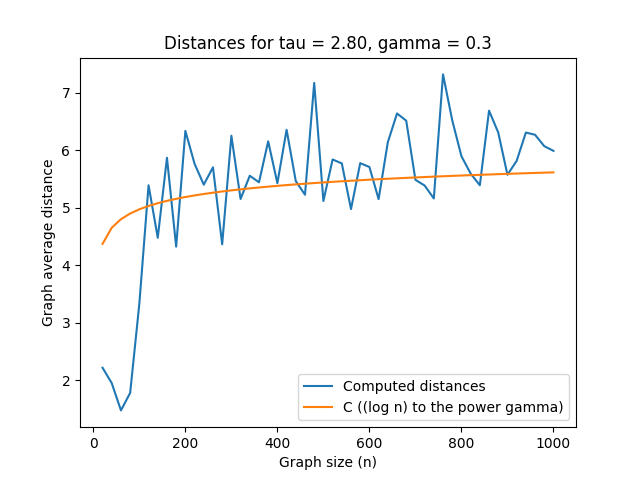
\includegraphics[scale=0.5]{log_gamma_03.png}
		\label{Fig1}
	\end{figure}
\end{minipage}
\begin{minipage}{80mm}
	\begin{figure}[H]
		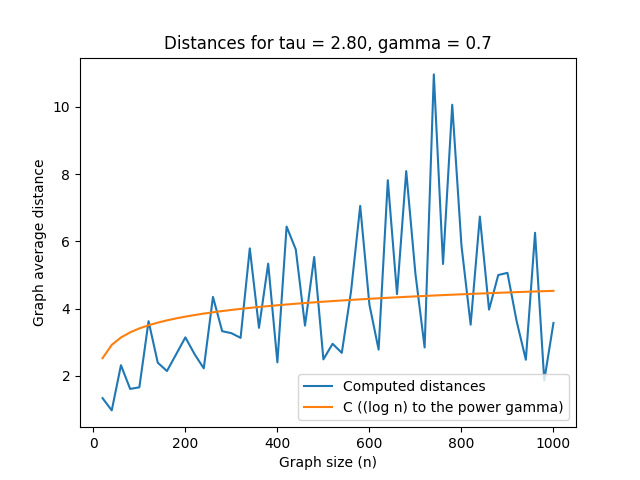
\includegraphics[scale=0.5]{log_gamma_07.png}
		\label{Fig2}
	\end{figure}
\end{minipage}

These plots are for the case when the truncation is harder and $\beta_n = o(1/\log\log n)$ (strictly speaking, here $\beta_n = 1/(\log n)^\gamma$). Here computations for each size were only conducted once so no smoothing is used for empirical (mean) graph distances plot. It also allows us to demonstrate that the behaviour of typical distances is only asymptotical and the addition of tight sequence in the main formula makes sense both theoretically and practically. We also show that it works as much for $\tau~\rightarrow~(3-)$ as for $\tau \rightarrow (2+)$.

\begin{minipage}{80mm}
	\begin{figure}[H]
		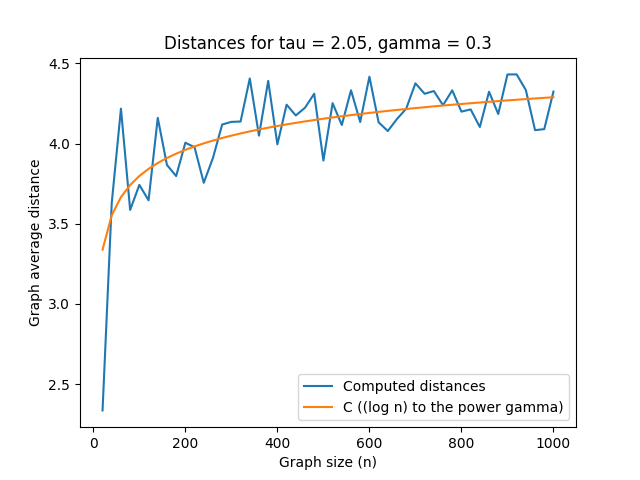
\includegraphics[scale=0.5]{log_gamma2_03.png}
		\label{Fig3}
	\end{figure}
\end{minipage}
\begin{minipage}{80mm}
	\begin{figure}[H]
		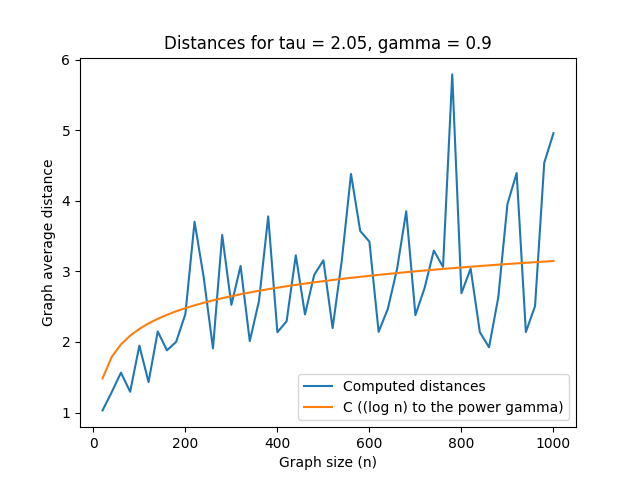
\includegraphics[scale=0.5]{log_gamma2_09.png}
		\label{Fig4}
	\end{figure}
\end{minipage}

Similarly, we computed plots for softer trunctation when it does not interfere with ultra-small behaviour of the network. Results in that case provide rather good empirical evidence of the nature of such truncation.

\begin{minipage}{80mm}
	\begin{figure}[H]
		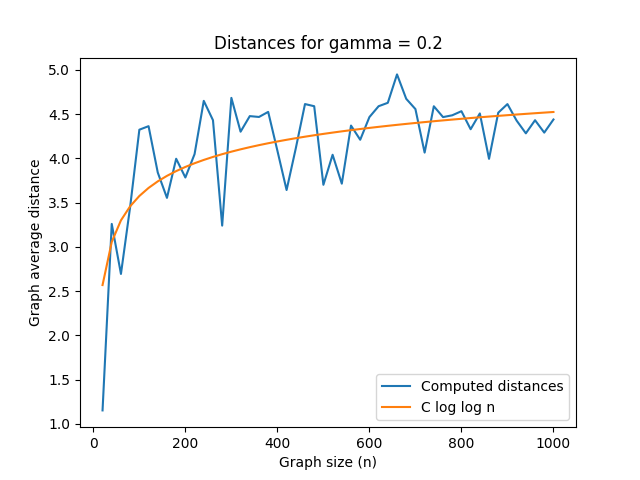
\includegraphics[scale=0.5]{loglog_gamma_02.png}
		\label{Fig5}
	\end{figure}
\end{minipage}
\begin{minipage}{80mm}
	\begin{figure}[H]
		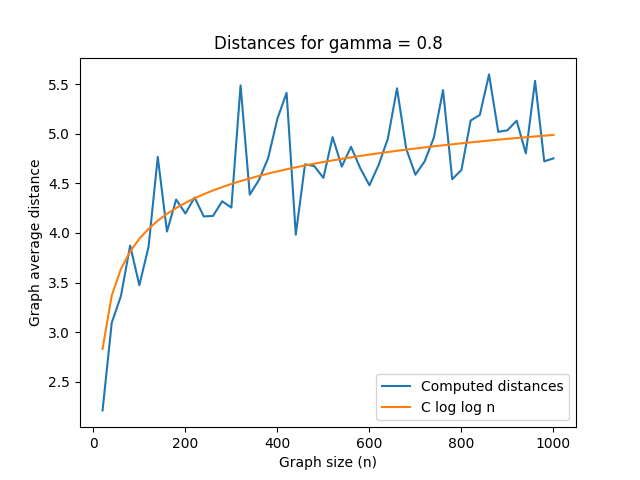
\includegraphics[scale=0.5]{loglog_gamma_08.png}
		\label{Fig6}
	\end{figure}
\end{minipage}


\addcontentsline{toc}{section}{References}
\begin{thebibliography}{9}

\bibitem{paper}
R. van der Hofstad, J. Komjáthy. \emph{When is a scale-free graph ultra-small?}. [Online] Available: https://link.springer.com/article/10.1007/s10955-017-1864-1

\bibitem{collab}
Newman, M .E .J. \emph{Scientific collaboration networks. I and II.} Phys. Rev. E 64(1), 016131–016132 (2001)

\bibitem{book_1}
R. van der Hofstad. \emph{Random Graphs and Complex Networks, Volume 1}. [Online] Available: http://www.win.tue.nl/\~{}rhofstad/NotesRGCN.pdf

\bibitem{book_2}
R. van der Hofstad. \emph{Random Graphs and Complex Networks, Volume 2}. [Online] Available: http://www.win.tue.nl/\~{}rhofstad/NotesRGCNII.pdf

	
\end{thebibliography}

\end{document}